\textbf{\textcolor{blue}{3.}} \Large
A partir del Ejercicio 2, muestra los registros de activación generados por la función con
la siguiente llamada.
\begin{lstlisting}
(ocurrencias '(1 2 3) '(1 2))
\end{lstlisting}

\textbf{Solución.} A continuación se muestran los registros
de activación por llamada recursiva, estos son \newline

Registro principal:
\begin{center}
        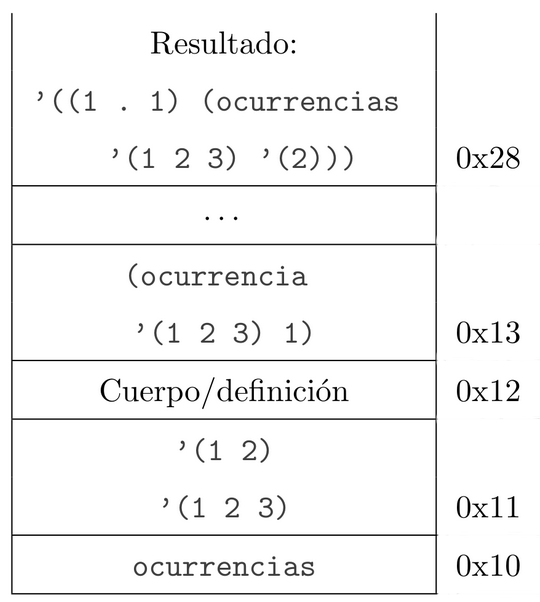
\includegraphics[scale=0.3]{./R1}
\end{center}


%%%%%%%%%%%%%%%%%%%%%%%%%%%%%%%%%%%%%%%%%%%%%%%%%%% TODO. No eliminar.
%%%%%%%%%%%%%%%%%%%%%%%% Primer Registro:
%\begin{table}[h]
%        \centering
%        \renewcommand{\arraystretch}{1.5}
%        \begin{tabular}{ | c | c }
%                         Resultado:                       &     \\
%                         \code{'((1 . 1) (ocurrencias }   &     \\
%                         \code{          '(1 2 3) '(2)))} & 0x28\\
%                         \hline
%                         $\dotsm$                         &     \\
%                         \hline
%                         \code{(ocurrencia }              &     \\
%                         \code{'(1 2 3) 1)}               & 0x13\\
%                         \hline
%                         Cuerpo/definición                & 0x12\\
%                         \hline
%                         \code{'(1 2)}                    &     \\
%                         \code{'(1 2 3)}                  & 0x11\\
%                         \hline
%                         \code{ocurrencias}               & 0x10\\
%                         \hline
%        \end{tabular}
%\end{table}

%Subregistro de activación 0x13
%\begin{table}[h]
%        \centering
%        \renewcommand{\arraystretch}{1.5}
%        \begin{tabular}{ | c | c }
%                         Resultado: \code{1}               & 0x27\\
%                         \hline
%                         $\dotsm$                          &     \\
%                         \hline
%                         \code{(+ 1 (ocurrencia '(2 3) 1))}& 0x17\\
%                         \hline
%                         Cuerpo/definición                 & 0x16\\
%                         \hline
%                         \code{1}                          &     \\
%                         \code{'(1 2 3)}                   & 0x15\\
%                         \hline
%                         \code{ocurrencia}                 & 0x14\\
%                         \hline
%        \end{tabular}
%\end{table}

%Subregistro de activación 0x17
%\begin{table}[h]
%        \centering
%        \renewcommand{\arraystretch}{1.5}
%        \begin{tabular}{ | c | c }
%                         Resultado:                        &    \\
%                         \code{ (ocurrencia '(3) 1)}       & 0x20\\
%                         \hline
%                         Cuerpo/definición                 & 0x19\\
%                         \hline
%                         \code{1}                          &     \\
%                         \code{'(2 3)}                     & 0x18\\
%                         \hline
%                         \code{ocurrencia}                 & 0x17\\
%                         \hline
%        \end{tabular}
%\end{table}
%
%Subregistro de activación 0x20
%\begin{table}[h]
%        \centering
%        \renewcommand{\arraystretch}{1.5}
%        \begin{tabular}{ | c | c }
%                         Resultado:                        &    \\
%                         \code{ (ocurrencia '() 1)}        & 0x23\\
%                         \hline
%                         Cuerpo/definición                 & 0x22\\
%                         \hline
%                         \code{1}                          &     \\
%                         \code{'(3)}                       & 0x21\\
%                         \hline
%                         \code{ocurrencia}                 & 0x20\\
%                         \hline
%        \end{tabular}
%\end{table}
%
%Subregistro de activación 0x23
%\begin{table}[h]
%        \centering
%        \renewcommand{\arraystretch}{1.5}
%        \begin{tabular}{ | c | c }
%                         Resultado:                        &    \\
%                         \code{0}                          & 0x26\\
%                         \hline
%                         Cuerpo/definición                 & 0x25\\
%                         \hline
%                         \code{1}                          &     \\
%                         \code{'()}                        & 0x24\\
%                         \hline
%                         \code{ocurrencia}                 & 0x23\\
%                         \hline
%        \end{tabular}
%\end{table}

\begin{multicols}{2}
Subregistro de activación 0x13
\begin{center}
        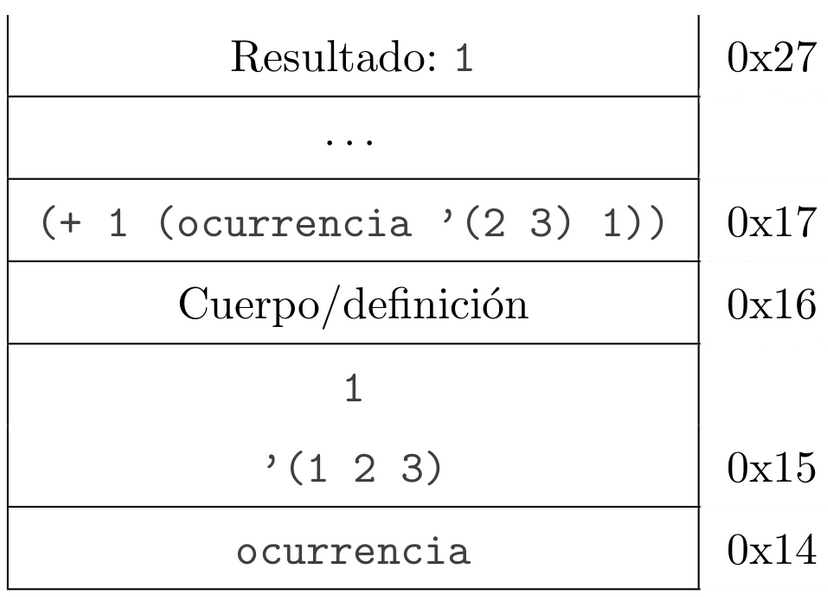
\includegraphics[scale=0.3]{./R2}
\end{center}

Subregistro de activación 0x20
\begin{center}
        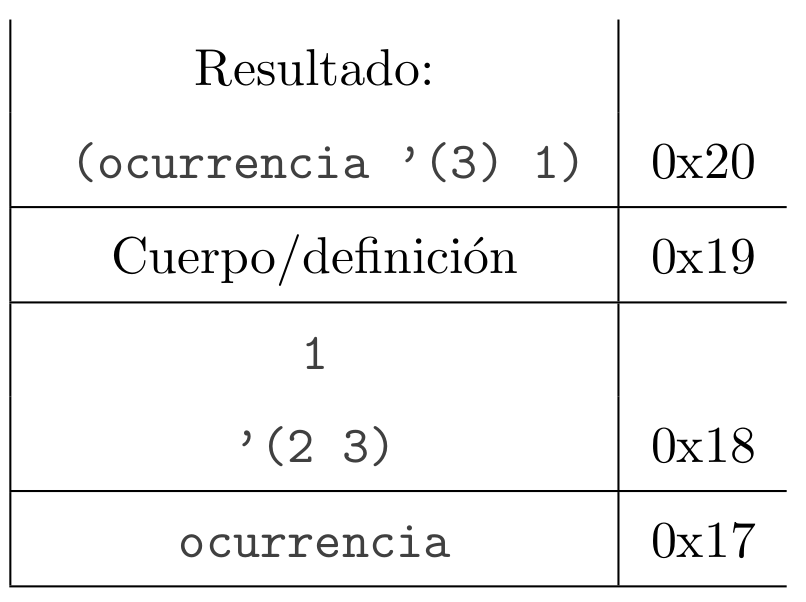
\includegraphics[scale=0.3]{./R3}
\end{center}

Subregistro de activación 0x17
\begin{center}
        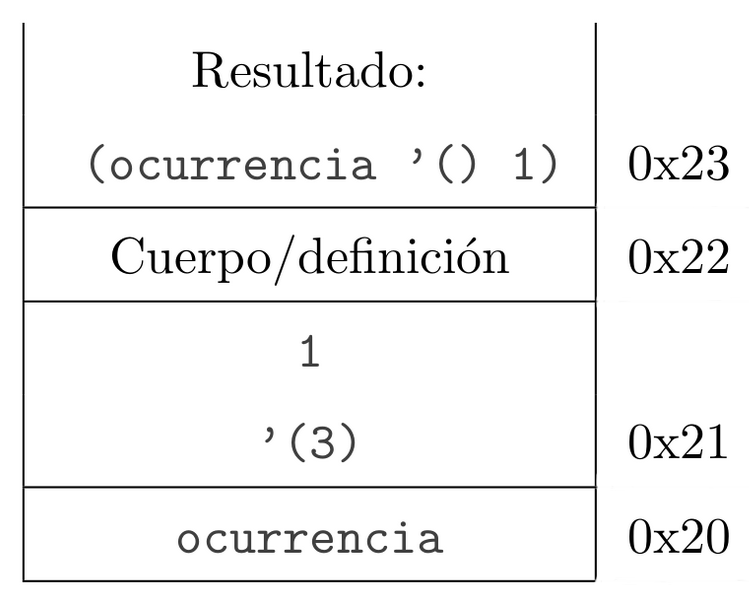
\includegraphics[scale=0.3]{./R4}
\end{center}

Subregistro de activación 0x23
\begin{center}
        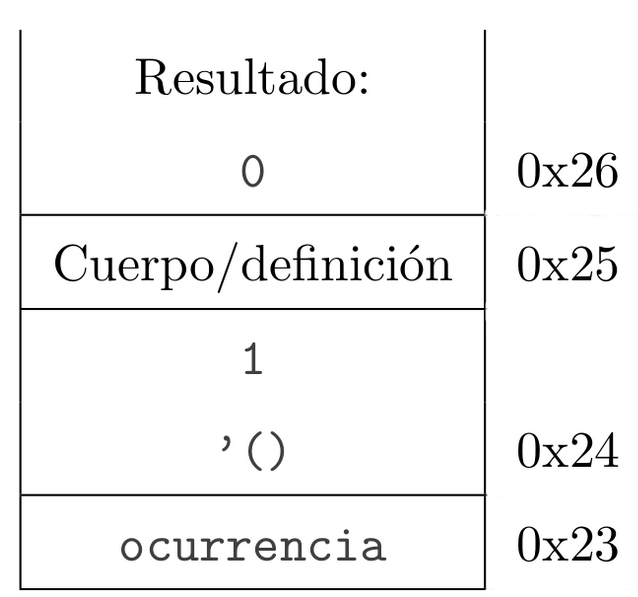
\includegraphics[scale=0.3]{./R5}
\end{center}
\end{multicols}

Segundo registro principal de la función \code{ocurrencias}:
